\chapter{System Designing}

\section{System Requirments to activate the system}

The system architecture is divided into three main components:

\begin{itemize}
    \item \textbf{Frontend:} The frontend is developed using React. It provides an interactive user interface for end-users to interact with the system.
    \item \textbf{Backend:} The backend is built with Django, a high-level Python web framework. It handles the application logic, user authentication, and serves as an intermediary between the frontend and the machine learning server.
    \item \textbf{Machine Learning:} The machine learning server is implemented using FastAPI. It processes and analyzes data, and exposes machine learning models via RESTful APIs.
\end{itemize}

\begin{figure}[h!]
	\centering
	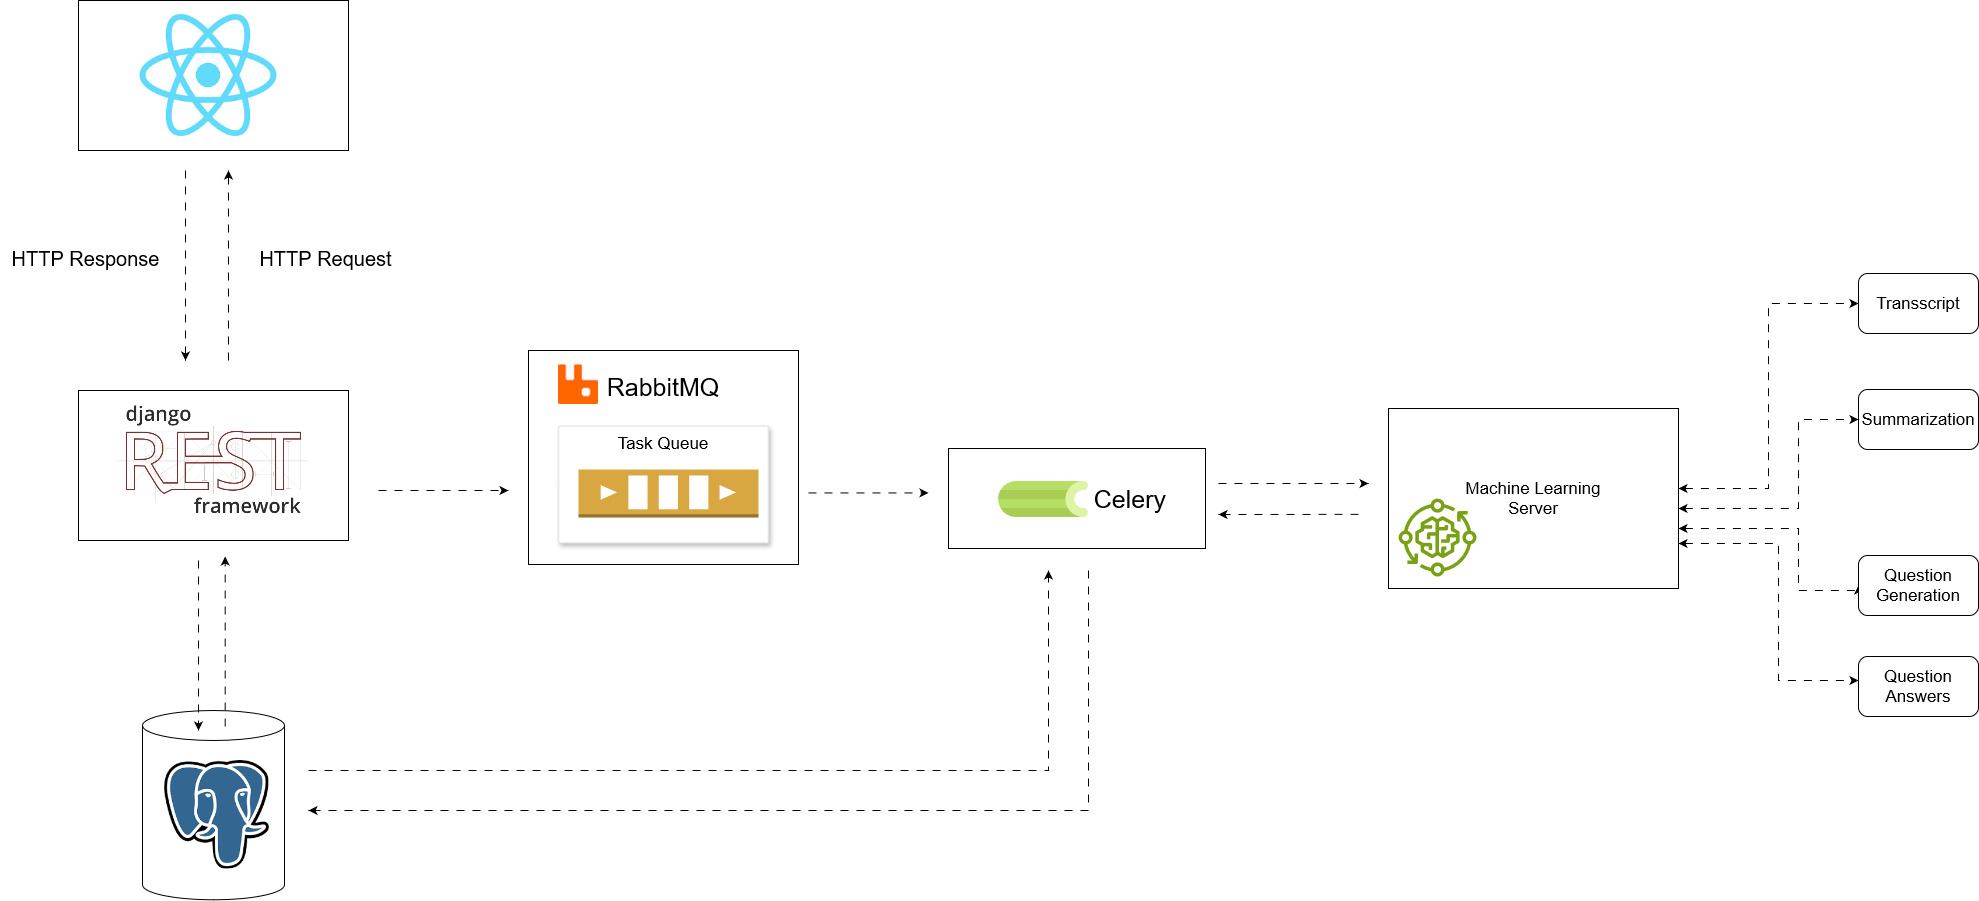
\includegraphics[max height=\textheight,max width=\textwidth]{figures/nerualearn.jpg}
	\caption{System Architecture}
\end{figure}

\subsection{Software Requirements}
\begin{itemize}
    \item \textbf{Node.js and npm:} Node.js and npm should be installed. They are required for building and running the React application.
    \item \textbf{React Build:} The React application must be built using the command \texttt{npm run build} to generate static files for deployment.
    \item \textbf{Python and Django:} Python and Django should be installed. The Django application must be properly configured and tested.
    \item \textbf{Database:} Set up the database (PostgreSQL) and should be configured correctly in the Django settings.
    \item \textbf{FastAPI:} FastAPI should be installed for serving ML models. The machine learning server must be properly configured and tested.
    \item \textbf{API Endpoints:} API endpoints should functioning correctly and are accessible by the backend.
\end{itemize}

\subsection{Hardware Requirements}
There are two sets of hardware requirements for the backend/frontend and the machine learning server.

\begin{itemize}
    \item \textbf{Backend and Frontend Server:}
    \begin{itemize}
        \item \textbf{Disk Space:} 1 TB (SSD class disk recommended)
        \item \textbf{Memory:} 4 GB
        \item \textbf{Processor:} 2 cores
    \end{itemize}
    \item \textbf{Machine Learning Server:}
    \begin{itemize}
        \item \textbf{Disk Space:} 1 TB (SSD class disk recommended)
        \item \textbf{Memory:} 16 GB
        \item \textbf{Processor:} 16 cores
        \item \textbf{GPU:} 24 GB
    \end{itemize}
\end{itemize}

\section{Code Screenshots Description}

\subsection{Machine Learning}
The implementation and code description of machine learning models is described in \hyperref[ch:modeling]{Chapter 5}

\subsection{Backend Core Functions}
	\subsection{API Endpoints}

\section{Application Screenshots}

\begin{figure}[h!]
	\centering
	
\includegraphics[max height=\textheight,max width=\textwidth]{figures/frontend/login mobile.png}
	\caption{Login Mobile}
\end{figure}

\begin{figure}[h!]
	\centering
	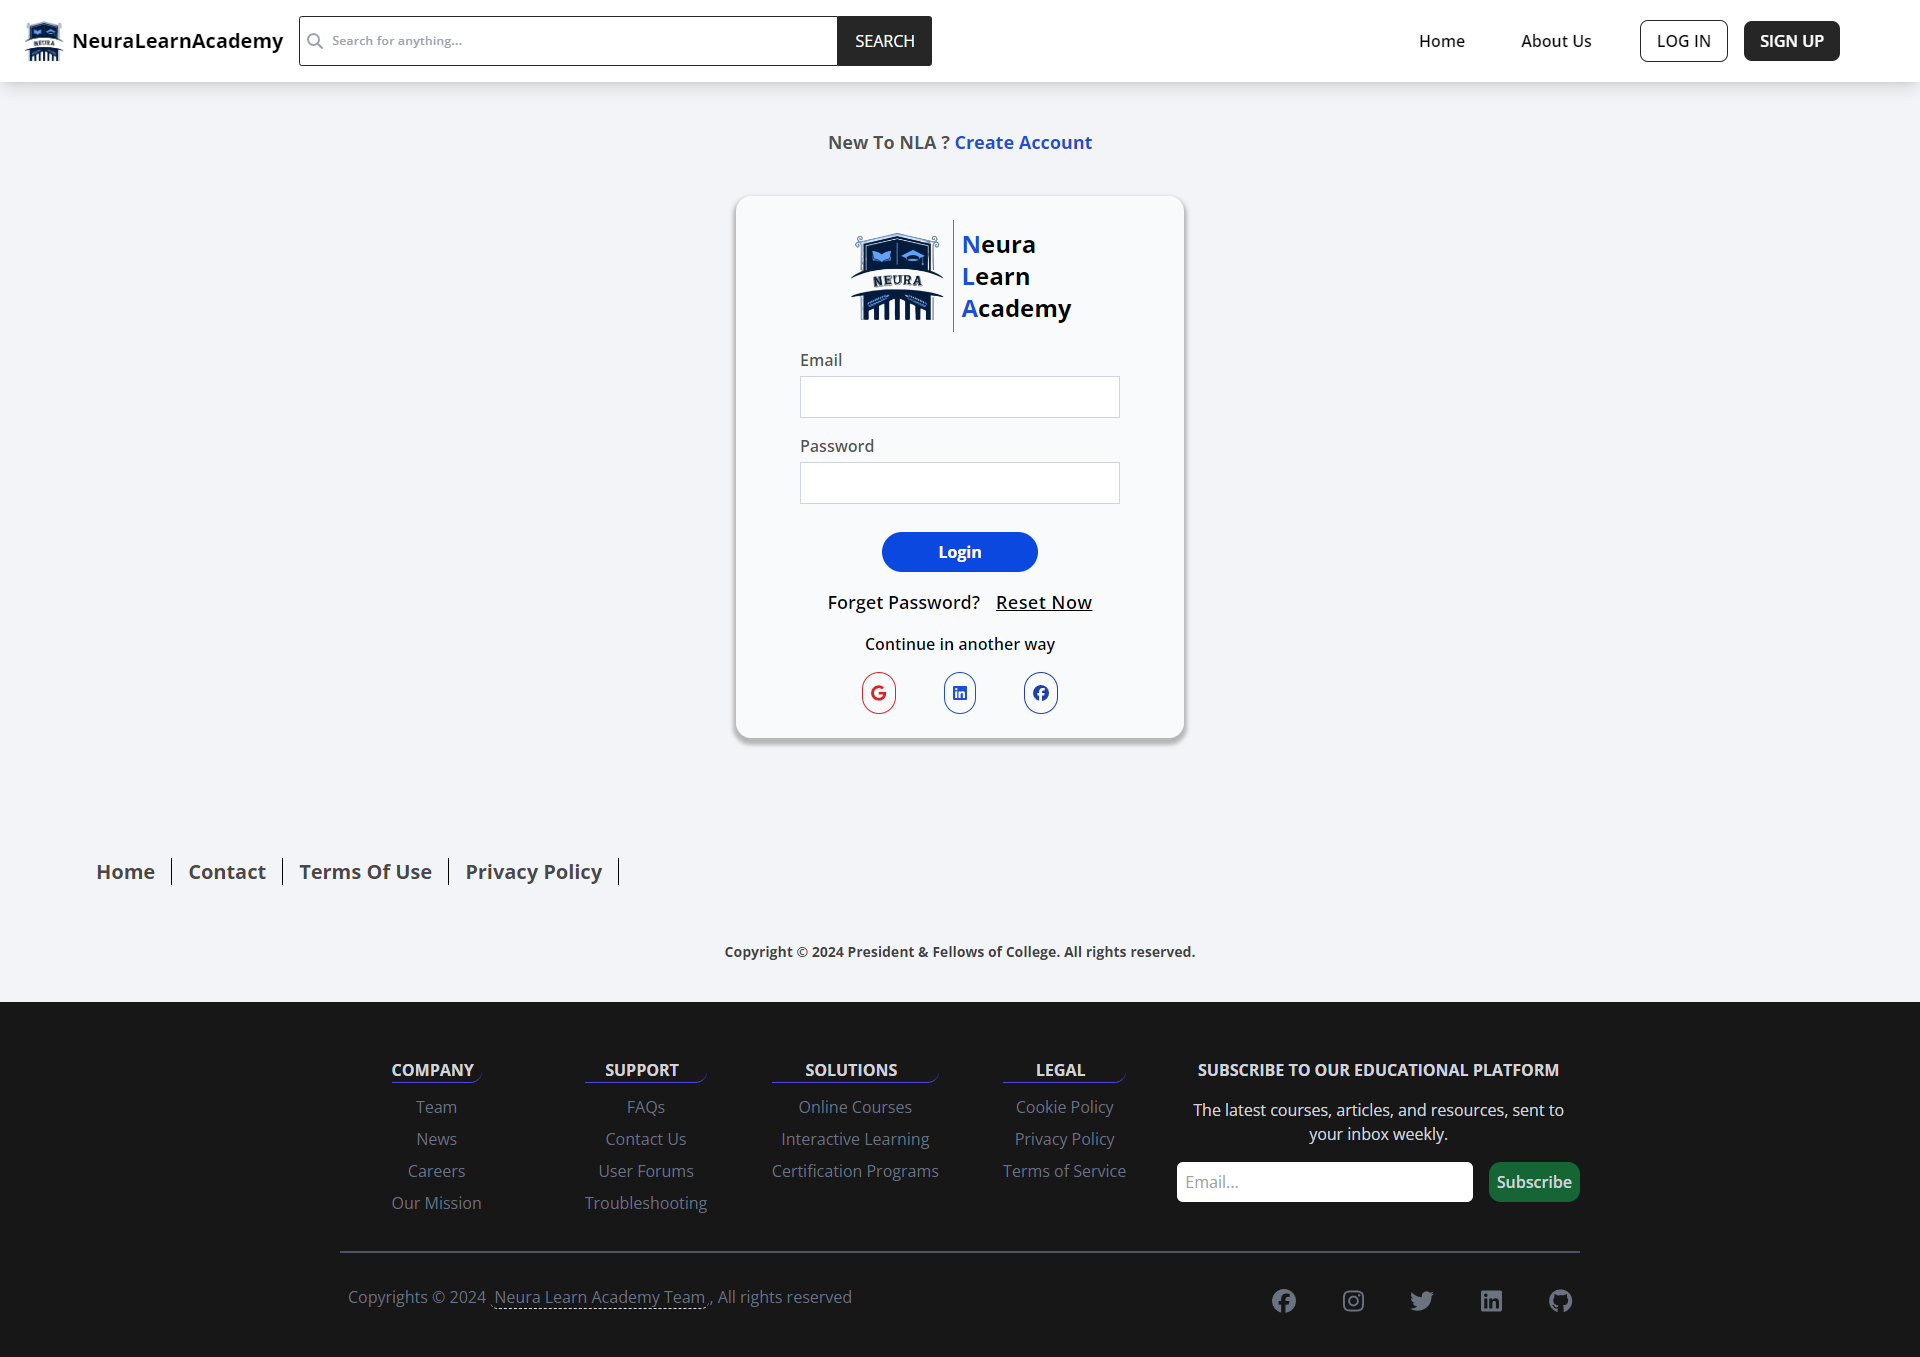
\includegraphics[max height=\textheight,max width=\textwidth]{figures/frontend/login.png}
	\caption{Login}
\end{figure}

\begin{figure}[h!]
	\centering
	
\includegraphics[max height=\textheight,max width=\textwidth]{figures/frontend/sign up mobile.png}
	\caption{Sign Up}
\end{figure}

\begin{figure}[h!]
	\centering
	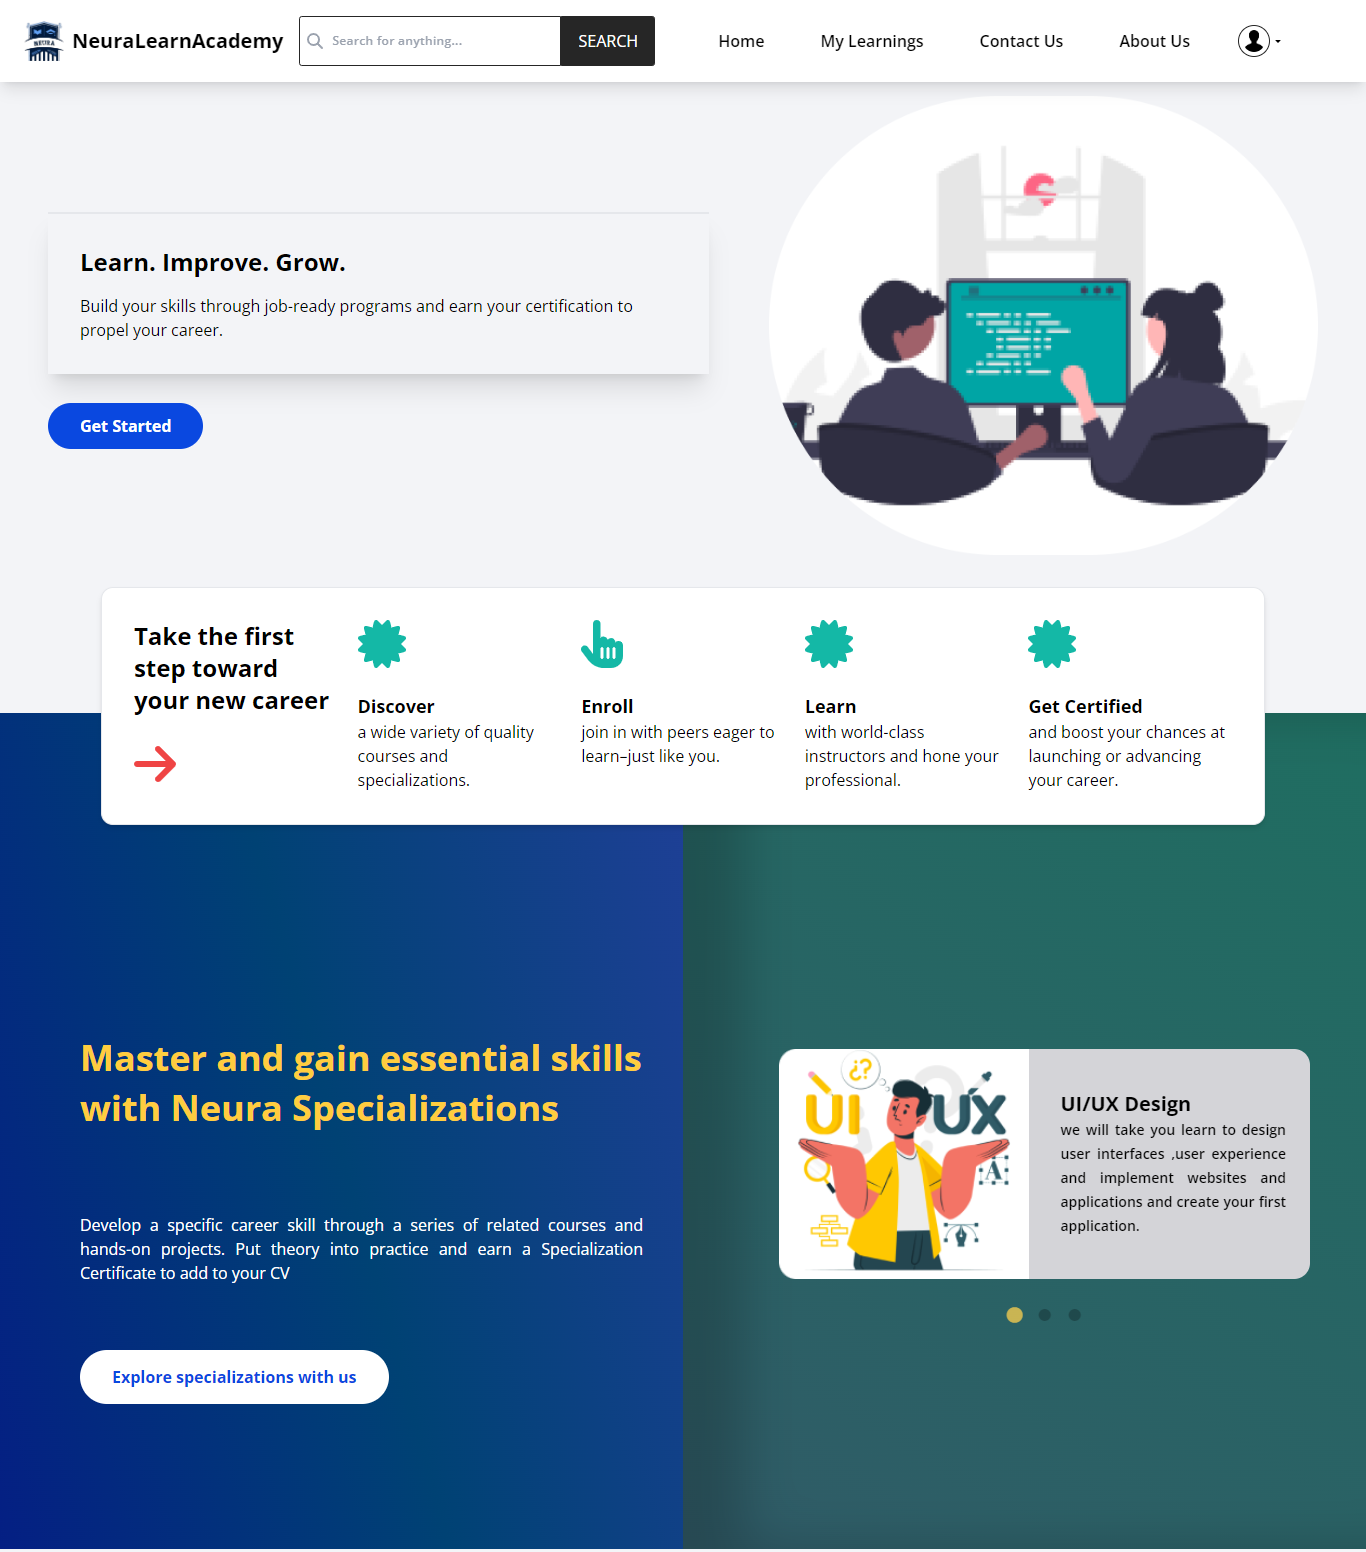
\includegraphics[max height=\textheight,max width=\textwidth]{figures/frontend/Homepage.png}
	\caption{Home page}
\end{figure}

\begin{figure}[h!]
	\centering
	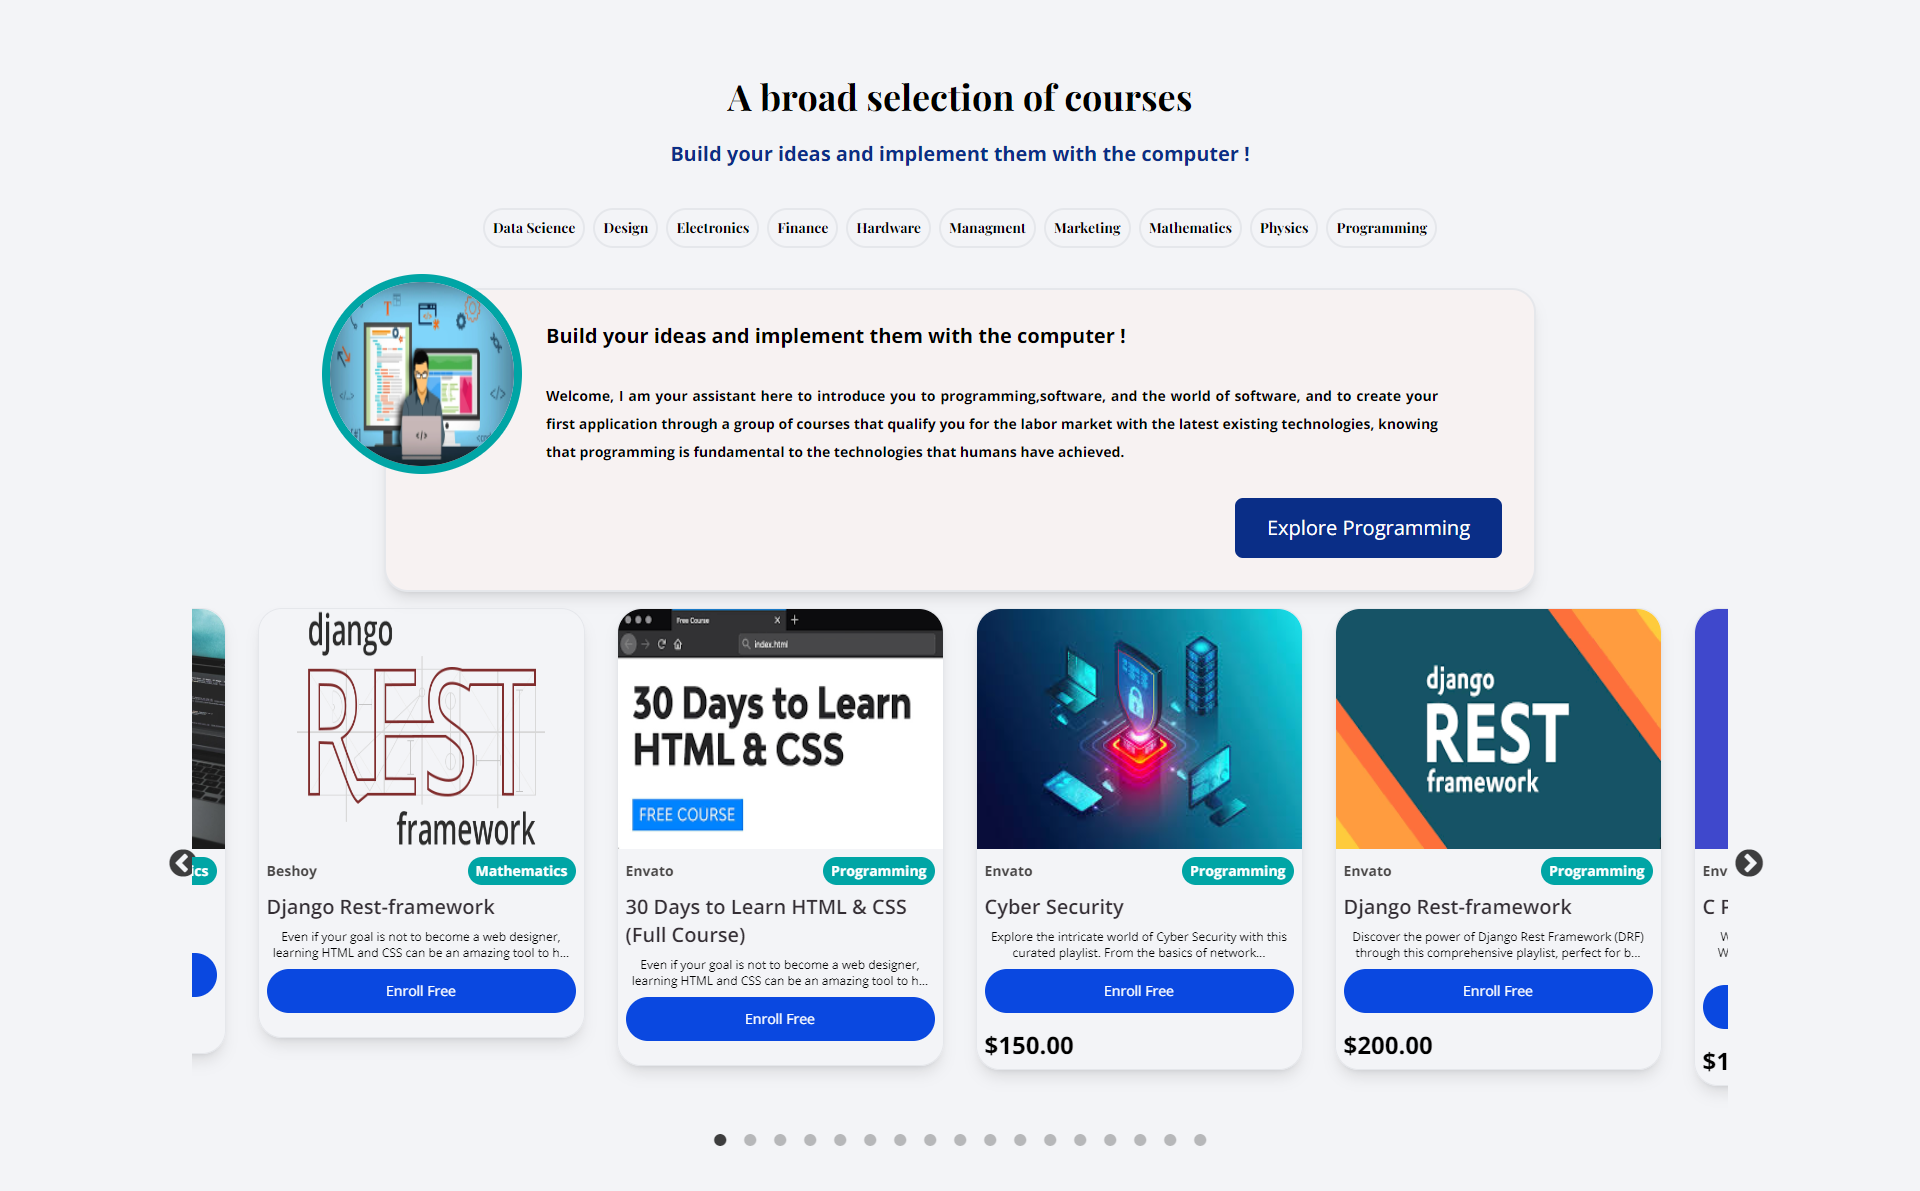
\includegraphics[max height=\textheight,max width=\textwidth]{figures/frontend/Homepage2.png}
	\caption{Home page 2}
\end{figure}

\begin{figure}[h!]
	\centering
	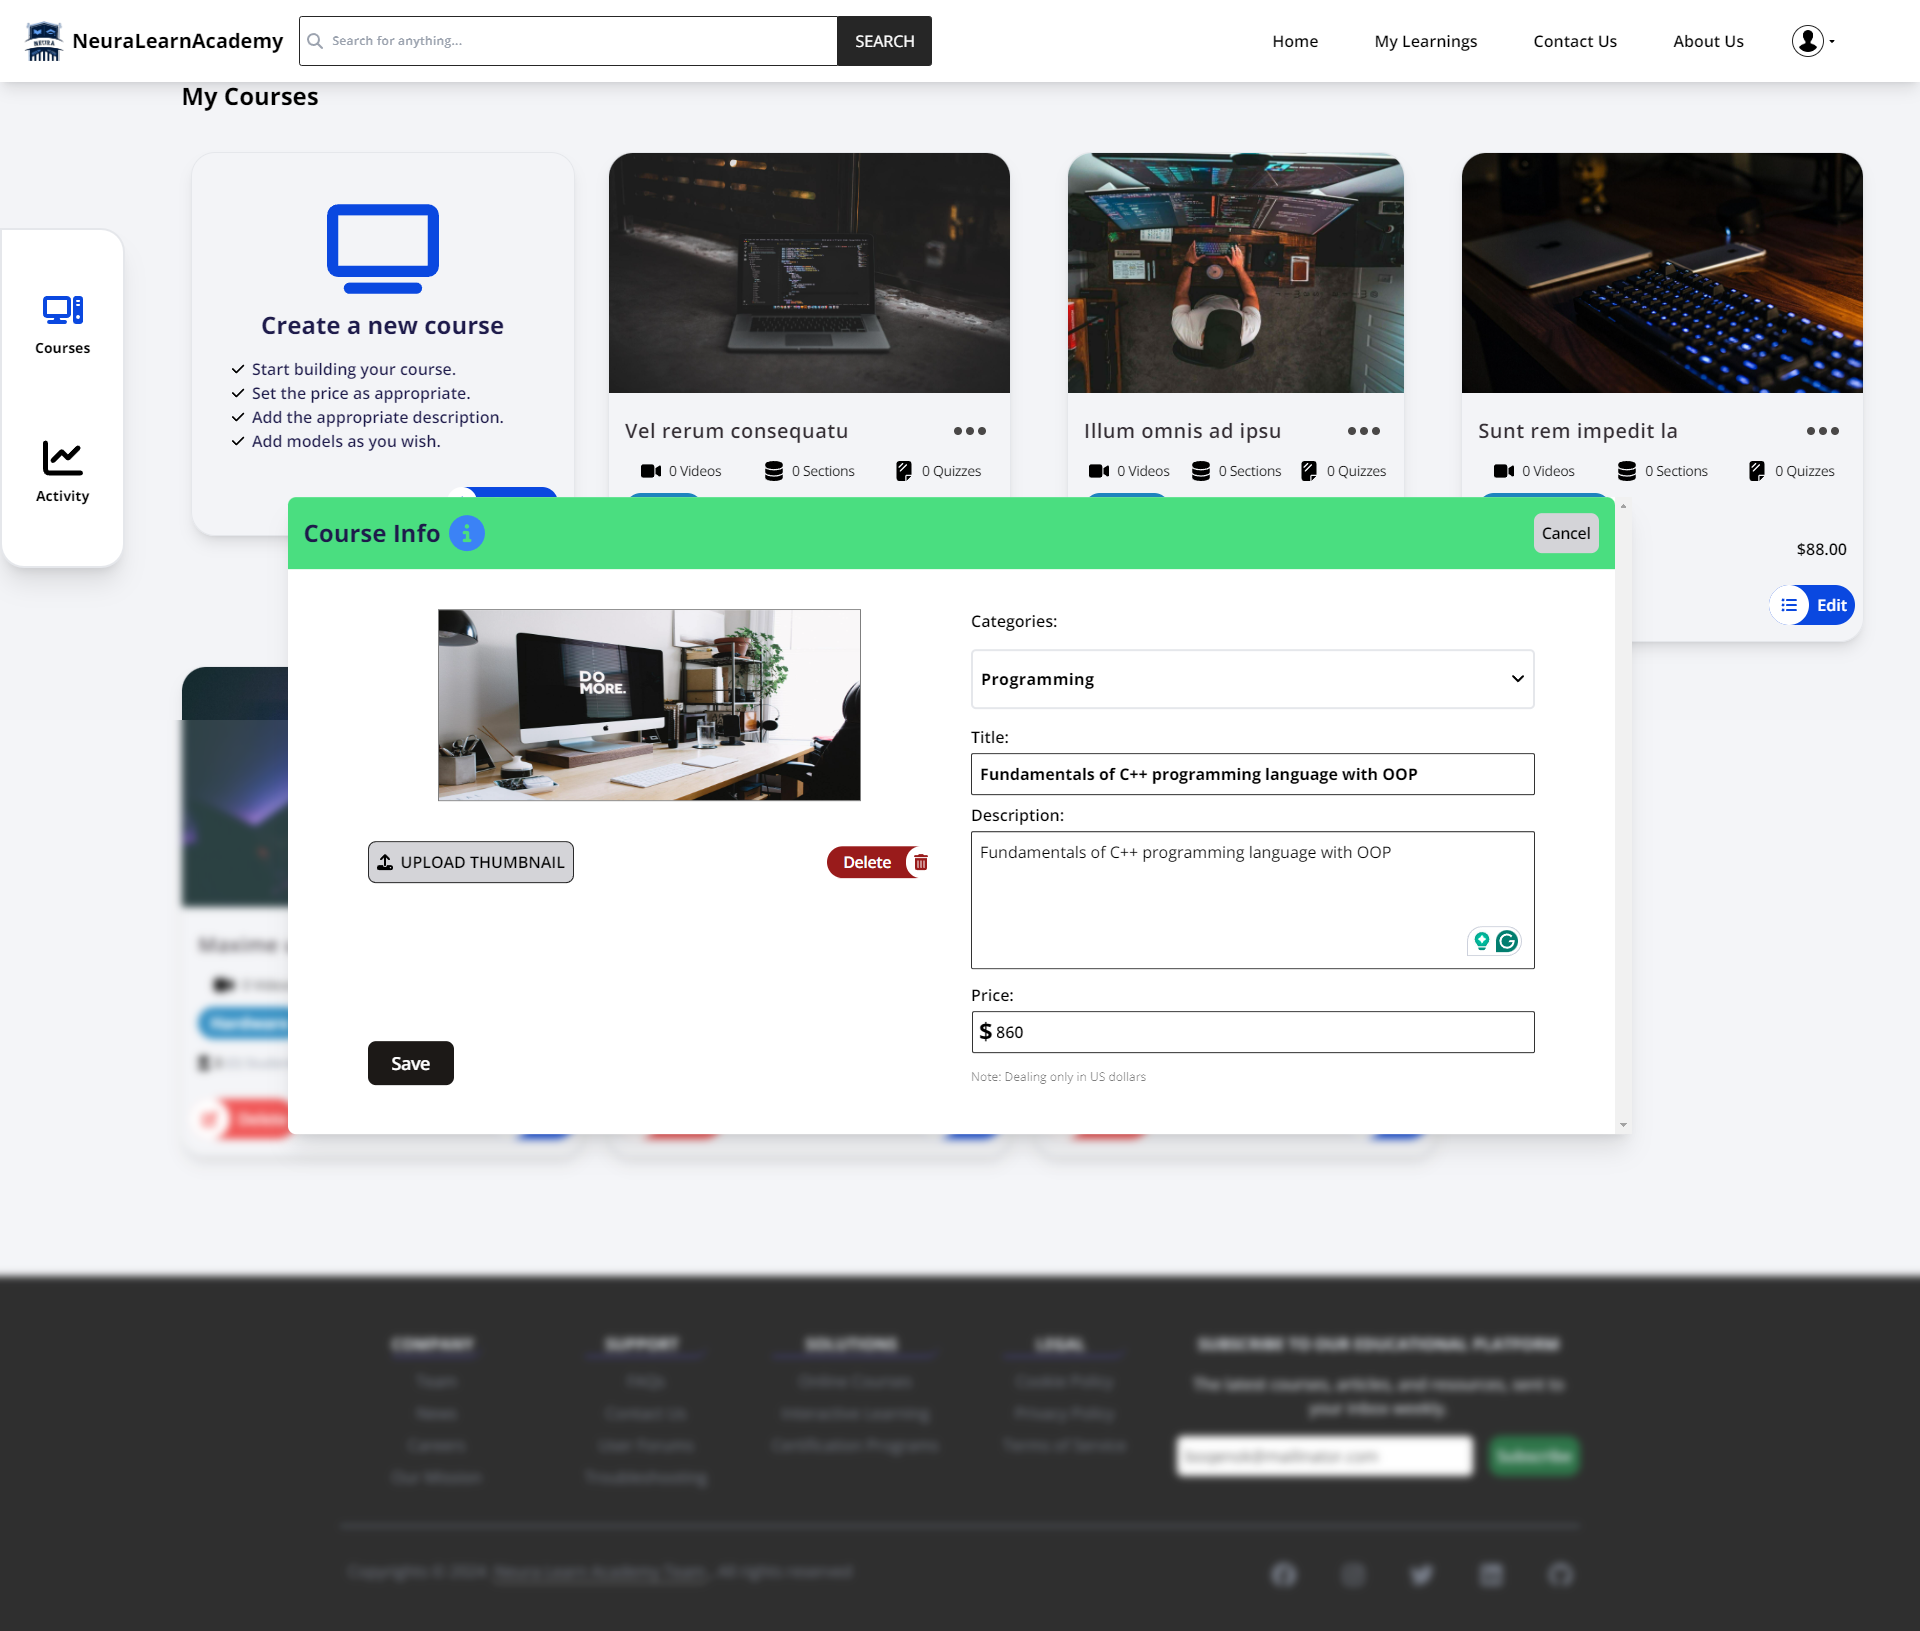
\includegraphics[max height=\textheight,max width=\textwidth]{figures/frontend/createcourse.png}
	\caption{Instructor Create course form}
\end{figure}